\documentclass[10pt,twocolumn]{article} 
\usepackage{latex8}
\usepackage{times}
\usepackage{graphics}
\usepackage{graphicx}
\usepackage{url}
\usepackage{color}
\usepackage{xspace}
\usepackage{mathptm}
\usepackage{algorithm}
\usepackage[noend]{algorithmic}
\usepackage{cite}
\usepackage{here}

%\setlength{\textheight}{9.5in}
%\setlength{\textwidth}{7in}
%\setlength{\columnsep}{0.125in}
%\setlength{\oddsidemargin}{-.25in}
%\setlength{\evensidemargin}{-.25in}
%\setlength{\topmargin}{-.5in}
%\setlength{\headheight}{0in}
%\setlength{\headsep}{.25in}

\renewcommand{\paragraph}[1]{\textbf{#1:}}

%\markboth{Draft - Do not redistribute}{Draft - Do not redistribute}
%\pagestyle{myheadings}
\newcommand{\comm}[2]{{\color{blue} (#1's comment: #2) }}
%\newcommand{\comm}[2]{}
\newcommand{\reply}[2]{{\color{green} (#1's comment: #2)}}
%\newcommand{\reply}[2]{}
\newcommand{\eat}[1]{}
\newcommand{\pr}[2][]{\ensuremath{P_{#1}\left[#2\right]}}
\newcommand{\dd}[2]{\ensuremath{\frac{d #1}{d #2}}}
\newcommand{\pow}[2]{\ensuremath{#1}^{#2}}

\newcommand{\PRT}{OptRT\xspace}
\newcommand{\fullPRT}{Optimized Routing Table\xspace}
\newcommand{\CRT}{ConsRT\xspace}
\newcommand{\fullCRT}{Constrained Routing Table\xspace}
\newcommand{\CRTNext}{$\mathrm{\CRT}_{\mbox{next}}$\xspace}

\pagestyle{plain}
\begin{document}
\title{Induced Churn as Shelter from Routing-Table
  Poisoning}
\author{
Tyson Condie, Varun Kacholia, Sriram Sankararaman, Joseph
M. Hellerstein, Petros Maniatis\\
\emph{UC Berkeley and Intel Research Berkeley}
}

%\date{}

\maketitle

\thispagestyle{empty}
\begin{abstract}
Structured overlays are an important and powerful class of
overlay networks that has emerged in recent years.  They are typically
targeted at peer-to-peer deployments involving millions of
user-managed machines on the Internet.  In this paper we address
{\em routing-table poisoning} attacks against structured overlays, in
which adversaries attempt to
intercept traffic and control the system by convincing other nodes to
use compromised nodes as their overlay network neighbors.  In keeping
with the fully-decentralized goals of structured overlay design, we propose a defense
mechanism that makes minimal use of centralized infrastructure.  Our
approach, {\em induced churn}, utilizes periodic routing-table resets,
unpredictable identifier changes, and a rate limit on
routing-table updates. Induced churn leaves adversaries at the mercy
of chance: they have little opportunity to strategize their positions
in the overlay, and cannot entrench themselves in any position that
they do acquire.  We implement induced churn in Maelstrom, an extension
to the broadly used Bamboo distributed hash table. Our
Maelstrom experiments over a simulated network demonstrate 
robust routing with very modest costs in bandwidth and latency, at
levels of adversarial activity where unprotected overlays
are rendered almost completely useless\footnote{This paper appears in NDSS~\cite{Condie2005}.}.
\end{abstract}

\Section{Introduction}
\label{sec:introduction}
In recent
years, the systems and networking communities have devoted significant
attention to techniques for coordinating large numbers -- millions
-- of computers in a decentralized fashion.   Originally motivated by
peer-to-peer filesharing applications, this research 
demonstrated massively distributed systems whose funding,
provisioning, and management are decentralized across numerous
parties with little shared trust.  More recently, this design
philosophy has been applied to a host of applications including
content distribution networks~\cite{Freedman2004}, geographic location
services~\cite{LaMarca2005}, file systems~\cite{Dabek2001},
monitoring systems~\cite{Bharambe2004}, document archives~\cite{Stribling2005}, and distributed query
processing~\cite{Loo2004}.  

Central to any of these systems is the notion of an {\em overlay
network}: a coordination mechanism for nodes running 
a distributed application to track each other, and to route messages
among themselves.  
Such large, open systems face constant \emph{churn},
the arrival and departure of nodes, as some fail,
hardware is replaced, connectivity changes, or software is upgraded.  
Much design and engineering are devoted to maintaining performance while
tolerating churn.

A particular class of overlays, \emph{structured overlays}
such as Chord~\cite{Stoica2003} and Pastry~\cite{Rowstron2001},
presents a hash table abstraction on top of a population of networked
computers.  Each participating node in the overlay has an ID from
a large identifier space, and is responsible for handling
messages addressed to an extent of the identifier space around its own
ID.  In order
to route messages in the overlay,
every node maintains a
routing table of ``links.''  The set of nodes and links in the system 
forms a structured network graph, over which
ID lookups can be routed to the responsible node efficiently,
even as the network churns.  When used to store data, structured
overlays are often called \emph{distributed hash tables} (DHTs), though many
structured overlay applications do not require storage.

An adversary who can subvert overlay routing can 
modify the overlay's behavior and hurt applications:
for example, she can convince a
correct (i.e., ``good'') node to redirect an outgoing link to
her, thereby \emph{poisoning} its routing table.  
All lookups routed via that link will end up in the adversary's
control; she can forward them or respond to them as she wishes.  This
has been called \emph{routing-table poisoning} or
an \emph{eclipse attack} in the literature.  
Once an adversary poisons a good node's routing table, she can {\em amplify}
that poisoning by intercepting the good node's maintenance
traffic, and convincing the node to update its routing table to
include additional compromised neighbors (Section~\ref{sec:eclipses}).

\paragraph{Previous Proposals}
Previous defenses against eclipse attacks have typically involved the
use of a trusted third party that regulates indirectly how nodes
partition the ID space, for example, by authoritatively assigning
IDs to nodes~\cite{Castro2002}.  The intuition is that if the
adversary's node IDs are chosen uniformly at random by an uncompromised
authority, then even the adversary receives
responsibility of an ID space share that is proportional to the number
of her nodes. She can therefore affect the system only in proportion to
her presence.
Centralized, globally
trusted certification authorities can be burdensome and difficult to
administer~\cite{Davis1996}, especially when multiple, mutually
distrusting administrative domains are involved.  However, they can offer
relief from rampant adversarial activity such as the use of forged,
throwaway identities (also known as Sybil
identities~\cite{Douceur2002}).

Note that defenses against Sybil attacks do not mitigate the threat of
amplification once a compromised node is chosen as a neighbor.  This
risk has become more important in recent, highly optimized structured overlays,
which make aggressive use of routing-table updates not only to address
churn in the network,
but also for performance optimizations such as latency
minimization over lookup paths through the graph~\cite{Gummadi2003b,Rhea2004}.

\paragraph{Our Contribution}
In this paper\footnote{An extended version of this paper can be found as
  a technical report~\cite{Condie:EECS-2005-11}.  In that version, we
  undertake a
  preliminary analysis of induced churn, modeling a simple adversary
  strategy.  Further analysis is the subject of our future work.} we ask
  two questions.  First, can there be an
effective defense against route poisoning attacks with a simpler, less trusted,
 centralized component that is easy to audit and replicate? Second, can
there be a practical, implementable defense against \emph{eclipse attacks} that
addresses the performance optimizations used in recent structured overlays?  We
present techniques that answer both questions in the affirmative.

Specifically, we propose the use of \emph{induced churn}
as a defense against eclipse attacks, unconventionally casting churn as
a tool rather than a scourge.  Induced churn consists of three
techniques: \emph{periodic reset of routing tables} to less efficient but more
attack-resistant ones,  forced \emph{unpredictable identifier changes},
and \emph{rate limitation on routing-table updates}.  We argue that by never allowing the overlay to
quiesce, we rob the adversary of the opportunity to plan ahead on node
positioning prior to an attack, and of her
ability to entrench herself, amplifying her position over time.
We show that for a typical, well-tuned structured overlay we reduce
routing-table poisoning by an order of magnitude and increase the
probability of successful lookups by as much as a factor
of 5, while incurring a maintenance overhead of under 1 KBps at each
node, low enough even for home users over dial-up connections.
Induced churn is applicable to any overlay application
that requires node \emph{organization} without persistent storage (e.g., for
query processing, multicast, or network monitoring); however for storage applications where churn
imposes data migration, induced churn
might be less appropriate (see Section~\ref{sec:discussion}).

In Section~\ref{sec:background} we present relevant background on
structured overlays, routing threats against them, and some
previously proposed solutions that form the basis for our defenses.
Section~\ref{sec:design} presents the design of our induced churn
defense against eclipse attacks.  We evaluate our design in
Section~\ref{sec:evaluation}, with experimental results on
\emph{Maelstrom}, a prototype
implementation of induced churn as an extension of the Bamboo structured
overlay~\cite{Rhea2004}. Our evaluation measures the improved security of the system
as well as the performance hit caused by routing-table reset, unpredictable identifier changes, and rate-limited routing-table updates.
Further we explore extensions, possible limitations, and big-picture implications
of this work in Section~\ref{sec:discussion}.  Finally, we conclude with
related work and our future research agenda.  


\Section{Background}
\label{sec:background}
As background, we present a brief primer
on structured overlay networks.  We
then discuss the class of attacks that concern us, and previously-proposed
defenses, before introducing induced churn in Section~\ref{sec:design}.


\SubSection{Structured Overlay Networks}
\label{sec:structuredOverlays}
An overlay network is a virtual network implemented on top of an
established underlying network of routers; in our discussion we will
focus on Internet overlays. Applications running at participant
machines communicate along the edges of the overlay network using
unicast transport services provided by the underlying network -- in
our case, by IP. Therefore, a message over an edge of 
the overlay may traverse many edges (IP router links) in the
underlying network. The algorithms for choosing overlay
edges differ among overlay designs.

A structured overlay builds its topology according to a particular model
graph
structure such as a hypercube, a torus, a de Bruijn graph, etc.  To
facilitate this construction, overlay nodes take identifiers from a
large ID space $\mathcal{I}$, which is typically the range of a
cryptographic
hash function (e.g., SHA-1), and is chosen to be sufficiently large (e.g.,
$160$ bits or more) to minimize name
collisions.  Overlay nodes take random IDs from $\mathcal{I}$.  Then the canonical model graph structure chosen
for the overlay is embedded in the ID space and mapped to the
existing overlay nodes.

To effect this mapping, responsibility for ID space ranges is
partitioned among the nodes in the overlay at all times.  In our discussion we will
assume that each node is responsible for the IDs that are nearest to
it in $\mathcal{I}$ (Figure~\ref{fig:OverlayExample}); other partitioning
schemes are used in the literature, but the choice has no impact on
our techniques below.

\paragraph{API}
The interface to the structured overlay consists of a single {\tt
lookup(id)} call.  In response, the overlay must locate the IP
address of the node currently responsible for ID {\tt id}, typically by
routing a message to that destination.

\paragraph{Topology and Routing}
The overlay's network topology -- the mapping of the model graph
structure to overlay nodes and links -- is captured via the {\em routing table}
maintained at each participant node.  For concreteness, we use Pastry~\cite{Rowstron2001} as an example
here.  Pastry is relatively easy to describe, and our implementation in
Section~\ref{sec:evaluation} was done in the Bamboo overlay, which uses a
Pastry-based topology.

\begin{figure}
\centerline{\includegraphics{OverlayExample}}
\caption{An example ID space for a structured overlay, represented as a ring.
  The nodes maintaining the overlay are represented as white circles on the
  ring; for example, computer $A$ is represented as the circle with
  ID $h(A)=F893A$. Dashed ovals represent the
  ``responsibility'' of every node, in terms of the ID range it
  manages.  In this example, every node manages the range of IDs that
  are numerically closest to its own identifier.}
\label{fig:OverlayExample}
\end{figure}


Many structured overlay designs, including those of Pastry and Bamboo, begin with a
reinforced ring topology, in which every node maintains links to the
participant nodes whose IDs are closest in $\mathcal{I}$ -- usually a
fixed number of successors and predecessors.  These are sometimes
called the node's \emph{leaf set}.  To provide routing efficiency, the ring is then
augmented with a set of neighbors that provide long ``jumps'' in
$\mathcal{I}$.

The choice of
which faraway nodes to link to is implementation-dependent.  In Pastry (and Bamboo) faraway links are
chosen according to a prefix-hypercube topology and
node IDs are represented in terms of digits in base $2^b$, where usually
$b=4$.  Hypercube links are stored in
a routing table that is divided into $160/b$ rows and
$2^b$ columns.  
For a node with ID $\gamma$, the routing-table
entry $(i, j)$ ``points to'' an ID that shares its leading $i$ digits
with $\gamma$, has $j$ as its $(i+1)$-st digit, and ends in any suffix. 
To populate that entry, $\gamma$ picks such an ID randomly, looks up the responsible
node, and stores its address and ID in the table entry.  There may be many candidate nodes for
a table entry $(i, j)$,
particularly for small values of $i$.  For example, in
Figure~\ref{fig:OverlayExample}, node $F893A$ could have in entry
$(0,9)$ any node
responsible for IDs starting with $9$ (e.g., $91188$ or $9D0E6$).
Typically, a node routes {\tt lookup($\alpha$)} greedily.  If among all
neighbors, its own ID is the closest to $\alpha$, the node responds
directly; otherwise it forwards the lookup to the neighbor or
leaf-set member whose ID is the closest to $\alpha$.

\paragraph{Dynamics}
Since structured overlays are intended for dynamic environments where nodes come and
go frequently and unpredictably, every node monitors the state of
the nodes to which it links, replacing any that disappear.
Consider the example in which Pastry node $F893A$ detects that
node $F8389$, contained in its routing-table entry $(2,3)$, no longer 
responds to pings.  Then, node $F893A$ looks for another candidate to
fill entry $(2,3)$, by choosing some random suffix $X$ and issuing  
{\tt lookup(F83X)}. Any
returned node responsible for ID $F83X$ can fill the empty entry.
 
In addition to ensuring the liveness of neighbors,
some structured overlays perform routing-table updates  to optimize
performance over lookup paths; Bamboo
is one example.  In such
designs~\cite{Gummadi2003b,Rhea2004}, a node maintains for every entry in
the routing table a number of candidate neighbors.  
The node keeps track of any performance metric with regards to those
candidates and chooses the 
best node among them to link to (e.g., the one with the smallest network 
latency, or highest uptime, etc.)  For example, the Bamboo node with ID
$F893A$ repeatedly looks up IDs with prefix $F83$ and includes the discovered
nodes to a set of candidates for routing-table entry $(2,3)$.  It picks
the closest candidate in terms of network latency for that entry, but keeps 
the rest as backup in case the chosen candidate fails.


\SubSection{Eclipse Attacks}
\label{sec:eclipses}
We shift our attention to attacks
on overlay routing.
To begin the discussion, we consider the case
in which some nodes become instantaneously compromised by a
single adversary.  Clearly the adversary also controls the fate of all
IDs mapped to her nodes.  A less obvious but 
important implication is that ``good'' (i.e., uncompromised) nodes'
routing tables now point to some compromised nodes.  We define as 
the \emph{level of poisoning} of a good node 
the
fraction of its routing table occupied by compromised nodes.


Singh et al.~\cite{Singh2004} formalized a pattern of misbehavior called 
an \emph{eclipse} attack, which consists of the gradual poisoning of good nodes' 
routing tables with links to a conspiracy of adversarial nodes. Note
that multi-hop routing in the overlay allows adversaries to intercept lookups
whose source and destination are both uncompromised. Left unchecked,
the adversary can eventually control most communication between good
peers, thereby placing a stranglehold on the quality and fate of
applications using the overlay.  The pace at which an adversary
is able to increase her control depends on the number of attack vectors available.


\paragraph{Amplification} In addition to intercepting application lookups,
the adversary can intercept lookups used by the overlay to choose
neighbors; she can thus influence good nodes'
neighbor selection, amplifying her ability to intercept subsequent traffic.
In the Pastry example, when node $F893A$ updates
the routing-table entry $(2,3)$, it looks up $F83X$.  If the path of the a lookup passes through a
compromised node, the adversary can intercept the request and respond to
it as if she controlled $F83X$, returning one of her nodes with the nearest ID. This behavior 
pattern causes a feedback cycle, whose result is an increase in good nodes' level of poisoning 
with most update requests they make.

\begin{figure}
\centerline{\includegraphics{FakeLatency}}
\caption{
  The victim sends a ``Ping'' message to adversary node ``Bad
  2,'' which relays the message over a low-latency link to ``Bad 1,''
  which finally returns a spoofed-source ``Pong'' message to the
  victim, pretending to be ``Bad 2.''  Whereas the correct
  round-trip IP latency from the victim to ``Bad 2''
  would have been 200 ms, it is presented as 130 ms.  Such latency ``savings'' -- which can be obtained
  through unpublished routes (e.g., with
  RON~\cite{Andersen2001}) -- give the adversary a significant advantage in
  optimized routing.}
\label{fig:FakeLatency}
\end{figure}

To make matters worse, optimized structured overlays offer further attack
vectors to the adversary, since they bestow upon routing tables  more
``degrees of freedom.''  There, a node selects the
optimal node for each routing-table entry according to measurements it
performs between itself and the candidate nodes.  If
such measurements can be biased by the adversary, then she can cause a
victim node to give preferential treatment to her nodes.  For example,
an adversary with good network connectivity can use her
resources to exhibit unnaturally low
network latency, as shown in
Figure~\ref{fig:FakeLatency}.

\paragraph{Simple Defenses} The presence of
adversarial nodes is inevitable in any practical open system.  In a
structured overlay, these nodes control the fate of the IDs for which they are
responsible.  To mitigate the ability of the adversary to intercept
traffic destined for other IDs, Castro et al.\ proposed \emph{redundant routing}~\cite{Castro2002}:
the sender sends its lookup to all of its leaf-set neighbors, who 
forward each duplicate lookup to the destination independently, in largely
distinct paths. This approach trades bandwidth for a higher likelihood of 
message delivery, and can be worthwhile for a small subset of critical traffic. 
We will use it later for routing-table maintenance lookups, for example.

With respect to optimized overlays,
the same work suggests the use of
failure detectors for routing.  One such failure detector depends on the
uniform distribution of identifiers over the node population,
implemented via a central identifier certification authority.  When the
failure detector points out that a lookup response is suspicious, then a
\emph{constrained}, unoptimized routing table is used as fallback to resend
the same lookup request~\cite{Castro2002}.  Constrained routing tables
limit the choice of nodes for each routing-table entry to one candidate.
In the Pastry example, entry $(0,9)$ in the constrained routing table of
node $F893A$ points to a single ID: the one numerically
closest to $9X$ for a \emph{fixed} suffix $X$ that the node chooses.  Contrast
this to regular Pastry routing tables, where \emph{any} suffix $X$, a full
16-th of the ID space, would be admissible instead.  As long as a
node can locate the correct candidate for an 
entry -- perhaps via redundant lookups -- it can ensure that its
constrained routing-table poisoning is similar to the
adversary-controlled fraction of the node population.
By maintaining both routing
tables -- one optimized but easily corruptible, and one slow but more
robust -- we can get
good performance and secure routing.  In the induced churn design, described
next, we utilize this idea of dual routing tables, though in a slightly
different manner that does not require failure detectors.



\Section{Design}
\label{sec:design}
Our contribution in this work arises out of the observation that,
regardless of fallback routing, poisoning in optimized routing tables
increases over time.  Our goal is to ensure that the \emph{average}
poisoning of good nodes' routing tables remains low over time.  To
accomplish this, 
our proposal retains the idea of maintaining both constrained and
optimized routing tables~\cite{Castro2002}, but with a twist.  Instead
of using a failure detector to decide when to
use each table for regular lookups, we impose a
\emph{periodic reset} of the optimized routing table to the contents of the
constrained one, always using the optimized routing table for lookups.
Optimization starts anew after reset, but the adversary must poison
good routing tables again to maintain her foothold.  Intuitively,
we seek to induce the poisoning behavior illustrated in
Figure~\ref{fig:sawtooth}.  Assuming resets bring the optimized routing
table back to its baseline level of poisoning, the more frequent the
resets, the lower the poisoning averaged over time.

\begin{figure*}
\centerline{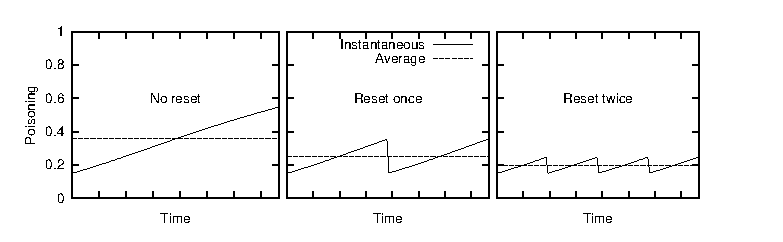
\includegraphics{graphs/equations/sawtooth}}
\caption{A graphical representation of routing-table reset, with
  increasing frequency from left to right graphs.} 
\label{fig:sawtooth}
\end{figure*}

Periodic reset can be helpful only if poisoning in the optimized
routing tables slowly increases over time; in Figure~\ref{fig:sawtooth}, the
slope of the ``sawtooth'' must be low.  In practice that is not always
the case, since ``eager'' update algorithms may optimize routing tables
fast, and preference to nearby nodes (in the network) can be
adversarially biased to converge always towards
greater poisoning.  To keep the slope low, we 
propose the \emph{rate limitation of routing-table updates}, since updates 
constitute the primary vector over which poisoning increase
is effected.  Instead of getting updates as fast as possible, we get
them at a fixed rate that does not change as network conditions or the
size of the overlay change.   Convergence to optimal connectivity
may be delayed as a result of this update rate limitation.  With it,
however, even a powerful adversary is prevented from bringing her
resources to bear to their fullest extent, reduced instead to the extent
admissible by our rate limits.

The last component of our contribution concerns predictability.  If the
adversary knows how optimized routing tables reset over time, then she
can conduct her attacks against content right before a reset
occurs. Furthermore, she can improve the deployment of her nodes (which
identifiers they have and which routing table they poison) using
knowledge of how good nodes' routing tables evolve with every reset.  We
deprive the adversary of this source of knowledge with
an \emph{unpredictable ID assignment}.  At every reset, every node picks a
new random ID and positions itself to a different part
of the topology, enforcing the same behavior on nodes in its own routing
tables.  If
good nodes ``move'' continuously, the adversary cannot attack them in
the same way after every routing-table reset; if all nodes, including
adversarial ones, must change their identifiers periodically (or face
disconnection from good nodes), then the adversary cannot hold on to
or improve upon advantageous positions in the
overlay.

We next describe a design that implements this basic intuition in
structured overlays.
Our design is generic and can be applied to any
specific structured overlay.  In Section~\ref{sec:evaluation} we describe a
particular implementation of induced churn for
Bamboo~\cite{Rhea2004}.
At a high level, our design consists of a common source of randomness to
reduce the predictability of the underlying overlay
(Section~\ref{sec:unpredictability}), functionality for computing and
validating fresh identifiers using this source of randomness
(Section~\ref{sec:identifiers}), machinery for effecting and enforcing
churn  (Section~\ref{sec:churn}), and a
mechanism for limiting the rate of routing-table updates
(Section~\ref{sec:rateLimitation}).  In
Section~\ref{sec:Optimizations}, we
present some extensions and optimizations to this basic design.


\SubSection{Timed Randomness Service}
\label{sec:unpredictability}

Our design relies on a \emph{timed randomness service}.
Periodically -- on the order of seconds -- this service
generates a fresh random number, which it places into a signed
\emph{randomness certificate} of the form [Timestep, Random].  The
service returns the current or any recent
randomness
certificate to anyone who asks, via some simple
transport mechanism, e.g., over HTTP.

This is a relatively simple service and  can be implemented in
a variety of ways.  A straightforward implementation would be centralized,
requiring little more than a well-managed but lightweight web server, with minimal storage
and a processor only strong enough to produce a signed random number
every few seconds or so.  It requires that all nodes have the
server's public key; this key may be distributed with the overlay software bundle, or 
via a network discovery protocol like DHCP or DNS. Here we assume that the randomness
server is available, uncompromised, and reachable with low latency
from all nodes.  These goals may be difficult to realize.  However, the reader should note
that the timed randomness service is light weight, easy to audit, and amenable to replication.
The ease of replication in particular alleviates the risk of DDoS attacks on the 
randomness service. In this paper we do not discuss the details of implementing a 
fully decentralized randomness server although we do explore alternative designs in
Section~\ref{sec:discussion}, and discuss the complexity-accountability trade-off for such a service.

\SubSection{Random Unpredictable Identifiers}
\label{sec:identifiers}

In this section we discuss the details of node identifier generation, and how it is done
in an unpredictable fashion.  It is typical for an overlay node to set its
identifier by hashing its IP address
(e.g., Chord~\cite{Stoica2003}).   We augment this construction with a
fresh, random nonce. To join the
overlay, or whenever it must reset its identifier, a node obtains the
appropriate random number from the randomness service.  It then computes
its new identifier by hashing its address and that number: $\mathit{newID} =
\mathrm{hash}(\mathit{Random} \| \mathit{IPAddress})$.  Given the
same random number, 
other nodes will be subsequently able to validate the computation of
this ID from the node's IP address.  These validations replace the
validation of centrally issued ID certificates, in a certification
authority-based design.

The choice of the appropriate random number -- that is, the timestep
to be requested from the randomness server -- is dependent on the
frequency with which identifiers must be reset.  We call the time
between identifier changes in our induced churn scheme an
\emph{epoch}, and express the length of the epoch in terms of timesteps
of the randomness service; we will explore the tuning of the
epoch length in Section~\ref{sec:evaluation}.  By convention,
the ``beginning'' of an epoch is the timestep of the randomness
service that is an integer multiple of the epoch length.  In other
words, at timestep $t$, current overlay IDs must be computed
using the random number issued by the randomness server at timestep
$t - (t \mathrm{\ mod\ } k)$, where $k$ is the number of timesteps
in an epoch. In Section~\ref{sec:staggering} we
refine this convention further.

\SubSection{Induced Churn}
\label{sec:churn}

Every node in our design maintains 
two kinds of routing state: an \fullPRT (\PRT) and a \fullCRT
(\CRT). The node uses its \PRT for all application lookup requests and
maintenance requests for the \PRT itself.  The node uses
the \CRT for all lookup requests that assist others to join the overlay,
either initially or after the end of an epoch, and to maintain the \CRT
itself. Lookups over the \CRT are performed redundantly to increase the chances that they
reach their intended destinations .

At the end of its epoch (i.e., every $k$ timesteps of the randomness
service), a node obtains the random number for its next epoch from the
service and uses it to compute its next identifier (Section~\ref{sec:identifiers}).  It then joins the overlay with that new
identifier; its join -- a lookup for the new identifier --
is routed redundantly over the \CRT of the nodes in the overlay.  When
the (re)joining node has acquired a new \CRT, 
it resets its \PRT to the new \CRT and abandons its old identifier.
It then begins optimizing its \PRT anew, until the end of the epoch.

Nodes evict from both routing tables those entries containing \emph{stale}
identifiers.  An identifier is stale if the random number used to
compute it is too old, that is,
$k$ or more timesteps earlier than the current randomness server's
time.  In this sense, nodes enforce a maximum lifetime of one epoch
length
on the nodes contained in their routing tables.



\SubSection{Update Rate Limitation}
\label{sec:rateLimitation}

We impose a limit on the rate at which updates are applied to a node's
routing tables in order to slow down the proliferation of malicious
entries.
When first joining the overlay or after
churning, a node starts a periodic update timer.  Whenever that timer
expires, the node issues an update request for each of its routing
tables to obtain up-to-date candidates for some randomly chosen table
entries.  
As described in Section~\ref{sec:eclipses}, for the \CRT the new candidate
node is found via a redundant lookup, and
is accepted into the entry if its identifier is numerically closer to the
entry's target than the existing link.
For the \PRT, the candidate node is found via a single-path lookup, and is
accepted if the entry was empty before, or if the candidate's
measurements on the
optimized network metric are better than all other known candidates for
the same entry.

Updates to both routing tables must be rate
limited, but update rates need not be the same for both
tables, though our prototype does use the same rate.
Nodes set the period of the update
timer according to a trade-off between system adaptability and desired
routing security;  more frequent updates improve responsiveness to highly
dynamic environments at the expense of security and possible
congestion~\cite{Rhea2004}, whereas less frequent updates are cheaper,
facilitate defense against eclipse attacks, but hinder responsiveness to
topology change.

Update rate limitation should apply to single-entry updates; for some
structured overlay
update mechanisms that update entire groups of entries in one go, further
refinement is required.  For such ``bundled'' updates, we randomly
drop some of the update contents.   We thus \emph{shield} the recipient
group of entries in the target routing table from being completely
poisoned in one fell swoop due to an unfortunate choice of lookup
path. Instead, to poison many routing-table entries, a node must make many unfortunate
update choices.


\SubSection{Optimizations}
\label{sec:Optimizations}

\begin{figure*}
\begin{tabular}{cc}
\begin{minipage}{3.5in}
%\footnotesize
\textbf{function} staggeredChurn()
\begin{algorithmic}[1]
\STATE $\mathit{LeafSet} \leftarrow \mathit{LeafSet}_\mathit{next}$

\STATE $\mathit{OptRT} \leftarrow \mathit{ConsRT}_\mathit{next}$

\STATE $\mathit{ConsRT} \leftarrow \mathit{ConsRT}_\mathit{next}$

\STATE $\mathit{ConsRT}_\mathit{next} \leftarrow \mathit{LeafSet}_\mathit{next} \leftarrow null$

\IF {$\mathit{LeafSet} = null$}

\STATE Rejoin network anew

\ENDIF

\STATE Call $\mathit{staggeredChurn()}$ in time $\mathit{epochLength}$ 

\STATE Call $\mathit{precomputeNeighbors()}$ in time
$\mathit{epochLength} - \delta$

\end{algorithmic}
\end{minipage}&\begin{minipage}{3.5in}
%\footnotesize
\textbf{function} precomputeNeighbors()
\begin{algorithmic}[1]
\STATE $\mathit{peer} \leftarrow \mathit{lookup(myNextID)}$
\STATE $\mathit{LeafSet}_\mathit{next} \leftarrow \mathit{null}$
\STATE $\mathit{tmpLeafSet} \leftarrow \mathit{peer.getLeafSet()}$
\FORALL{$p \in \mathit{tmpLeafSet}$}
	\IF {$\mathit{nextChurnTime} < \mathit{expireTime}(p)$} 
		\STATE {$\mathit{LeafSet}_\mathit{next}.\mathit{add}(p)$}
	\ENDIF
\ENDFOR
\STATE Populate $\mathit{ConsRT}_\mathit{next}$ for identifier
$\mathit{myNextID}$
\FORALL{$p \in \mathit{ConsRT}_\mathit{next}$}
	\IF {$\mathit{nextChurnTime} < \mathit{expireTime}(p)$} 
		\STATE Remove $p$ from $\mathit{ConsRT}_\mathit{next}$
	\ENDIF
\ENDFOR 
\end{algorithmic}
\end{minipage}
\end{tabular}
\caption{Pseudocode for the staggered churn and routing-table precomputation algorithms.\label{fig:pseudocode}}
\end{figure*}
Up to this point, we have presented a simple design.
In this section we complicate it slightly to
introduce two important optimizations that allow induced churn
in practice, without undue sacrifices in performance.  The resulting
pseudocode appears in Figure~\ref{fig:pseudocode}.

\SubSubSection{Staggered Churn}
\label{sec:staggering}

If all nodes in the system churn every $k$-th timestep, then the system
will likely be very unstable and heavily loaded right around the global churn
time. It will also move from less poisoned to more poisoned
states uniformly, making it easy for the adversary to pick when to attack.
We now describe how to \emph{stagger} 
induced churn by partitioning the population into $G$
\emph{churn groups}, each churning at a different timestep.

We define churn groups according to nodes' IP addresses, for
example, by setting a node's group number to $(\mathrm{hash}(\mathit{IPPrefix})
\mathrm{\ mod\ } G)$.  $\mathit{IPPrefix}$ is an appropriately sized
prefix of the node's IP address, e.g., 24 bits, long enough to ensure a
reasonably uniform group size distribution, but short enough to prevent
the adversary from changing her nodes' churn groups by fiddling with the
highly spoofable low-order bits of IP addresses.

In order to stagger churn, we must make minor modifications to the
identifier mechanisms described in Section~\ref{sec:identifiers}.  The
randomness server timestep when a node must switch identifiers is no
longer the same for all nodes, but is offset by the group number.
A node in group $g \in [0, G)$, must switch identifiers at all timesteps $t$ where
$t \mathrm{\ mod\ } k = gk/G$.  At timestep $t$, current, non-stale
identifiers of group $g$ must use the random number of timestep $(t -
((t - gk/G) \mathrm{\ mod\ } k))$.

A related implication of staggered churn is that different entries in
routing tables become stale at different times, and are verifiable
with different random certificates from the server.  To simplify
management of identifier expiration without overloading the randomness
server, nodes piggy-back the related randomness certificate with any
transfer of node identifiers during maintenance or other
identifier exchanges.  For the same reasons, nodes cache randomness certificates
for as long as they have related node identifiers in their routing
state.  With these small optimizations, a node need contact the
randomness server directly only once every epoch to obtain
the random number it needs before churning; it can also use
that opportunity to synchronize its clock to that of the server at
timestep granularity.  Since we expect timesteps to last a few
seconds, even high Internet round-trip times would allow fairly good time
synchronization of nodes with the randomness service for the duration of
an epoch.


\SubSubSection{Routing State Precomputation}
In the basic design of Section~\ref{sec:churn}, a node joins the overlay
with its new identifier at the beginning of each epoch.  While a node
is joining, it is unavailable for handling lookups.  To reduce the
impact of this regular occurrence, we allow nodes to \emph{precompute}
their next routing state.  When the epoch
boundary arrives, the node can immediately switch its leaf set, \CRT, and \PRT
to the precomputed routing state, making for a smooth transition.  If
the node has been unable to precompute its new routing
state on time, it joins with the new identifier as before.
This optimization requires that a
node know its next identifier ahead of time.  To
allow this, we \emph{shift} the mapping from randomness service timesteps to
epochs:  the random nonce for group $g$'s current epoch at
timestep $t$ is that issued at $T_g = (t - k - ((t - gk/G) \mathrm{\ mod\ }
k))$; the random nonce for group $g$'s next epoch is
$T_g + k$.

With routing state precomputation, at any given time a node maintains a
total of three routing
tables: a \fullCRT (\CRT), an \fullPRT (\PRT), and a speculative \fullCRT for the
next epoch (\CRTNext).
A node populates \CRTNext using its current
\CRT, by going through the motions of a join operation with its next identifier,
without actually changing any other node's routing tables: it looks up
its next identifier in the overlay to discover what
its leaf set and \CRT would be for that next
identifier.  This discovery is different for every structured overlay design.  In
Bamboo, for example, the node forwarding the newcomer's join lookup at every hop
sends the newcomer its routing-table row used to forward the lookup~\cite{Rhea2004}.
During precomputation, routing-table entries that will be stale by the time the node 
actually churns are excluded.  The precomputed \CRTNext is maintained using
periodic updates, just as the current \CRT is (see Section~\ref{sec:churn}). The careful
reader will notice that pruning nodes with IDs that expire prior to an induced churn point 
prefers nodes in groups immediately following the churning node's
group. To reduce this bias, nodes precompute the \CRTNext late in the current epoch. 
In the Figure~\ref{fig:pseudocode} pseudocode, this translates to making $\delta$ 
(last line of $staggeredChurn()$) as small as possible. 

Precomputation gives the adversary advance knowledge of 
where good nodes will be one epoch into the future.  This is an
important concern, making it undesirable to provide greater levels of
precomputation.  However, recall from
Section~\ref{sec:rateLimitation} that the adversary can only take
advantage of a
limited number of updates per epoch due to rate limitation.  For our single-epoch precomputation, the
adversary must decide whether to use her update budget to attack the
current epoch's \PRT, or to place her nodes so as to attack next epoch's
\PRT more effectively. Fortunately, even though she knows where her
nodes will be in the next epoch, just as good nodes do, she is still
limited to using an identifier for the duration of a single epoch only,
making such predeployment of assets limited in its utility.



\SubSection{Design Alternatives}
\label{sec:alternatives}
In this section we talk about the alternative designs for our defenses,
namely \emph{Forced Unpredictable Identifier Change} and
\emph{Periodic Resets}.

\SubSubSection{Alternatives for Forced Unpredictable Identifier Change}

Our design choice for forced unpredictable identifier change places the
responsibility of keeping time and producing unpredictability to a centralized
randomness server.  This is a reduction in central responsibility, compared to the
alternative of having a certification authority registering entities,
controlling the rate at which identifiers are issued, dealing with revocation,
etc.  An intermediate design point between the two would be to control
identifier unpredictability over entire groups of peers (according to some
grouping), reducing the state maintained at the server from the granularity of
individual addresses to that of groups.  In contrast to Maelstrom, this
approach is cheaper in terms of resources, but gives more responsibility
to the server, who can now bias group assignments.

Going in the opposite direction from our design choice towards less
centralized responsibility, we could distribute the task of controlling
unpredictability, for instance by using variants of shared coin flipping
schemes, such as that described by Cachin et al.~\cite{Cachin2000}.
The randomness server could thus be distributed over all peers or a set
of servers enjoying partial trust among the peer population.  This, for
instance, could be a task for the set of bootstrapping servers that most
overlays rely on.

Finally, an attractive fully distributed design we are considering
for future work would help an individual peer to ensure that identifiers
of peers it communicates with are determined in a manner unpredictable
to them and fresh within a time frame that the peer itself can track
alone.  The basic idea is to run an unpredictable logical clock per
peer.  At every timestep, each peer broadcasts the random value of its
clock to its neighbors.  A peer receiving clock values from its
neighbors hashes them together (e.g., in a Merkle hash tree) and
combines the result with its own previous clock value to produce a value
for the next timestep.  A peer's identity is cryptographically dependent
on the value of its local logical clock.

To prove to a neighbor that its identifier is relatively fresh and until
recently unpredictable, a peer traces a backward path from the clock
value that influenced its new identifier to a clock value issued by this
new neighbor some time in the past; this path follows backwards a
sequence of hashes and logical clock value broadcasts, e.g., tracing a
path from the new neighbor to the peer's old position in the overlay.
Since the neighbor remembers when it issued its own clock values (for a
short period in the past), it can estimate for how long the peer has
known its new identifier.  This is a simplified instance of the
coordination required for a distributed secure time stamping
service~\cite{Maniatis2002b}.  We are planning to explore the
overheads and potential benefits of such an aggressively decentralized
approach under heavy churn.

\SubSubSection{Alternatives for Periodic Reset}

We considered several alternatives for performing the periodic resets 
that trigger induced churn, including proximity-metric randomization, 
gang evictions, and selfish routing-table churn.  Proximity-metric 
randomization introduces error in the
measurement of the proximity metric used for routing optimization.  For the
example of point-to-point latency as the metric, we could randomize
several low-order bits of the measured latency per discovered peer.
Though coarse-grained differentiation among potential links
is still available, finer-grained comparisons of links change
unpredictably, causing proximity neighbor selection not to
converge always to the strictly closest neighbor  but, instead, to pick
at random from a larger set of otherwise nearby neighbors.  This
approach seemed awkward as it in effect tries to modify the proximity machinery
specific to Bamboo, while our solution is cleaner and applicable to any structured overlay.

Gang evictions would allow the peers currently occupying a neighborhood of the
logical overlay space collectively to decide the order of peer evictions and to
monitor joins. However, achieving consensus on evictions in a highly
decentralized, untrusted environment can be tricky and computationally
expensive, making this approach undesirable.

Selfish routing-table churning follows the similar philosophy of evicting entries
from a peer's routing table when those entries have exceeded a maximum
lifetime.  However, an identifier is not evicted from all routing tables
of correct peers at the same time.  As a result, though similar to our
eventual design, this
technique might lead to a continuous state of routing
inconsistencies~\cite{Liben2002short}.


\Section{Evaluation}
\label{sec:evaluation}

We evaluate induced churn against the goals of our system: defense against
eclipse attacks with acceptable performance.  First we describe Maelstrom, our prototype
implementation of induced churn built on top of Bamboo.  Then we measure
and compare the resistance of Maelstrom to poisoning, as well as its
overhead.


\paragraph{Implementation}
We have built Maelstrom as a secure extension to Bamboo, 
a fine-tuned, real structured overlay. Maelstrom is a secure router package, consisting
of about $5,000$ lines of Java source code.

The primary component in the Bamboo system is the Router, which
maintains 
a leaf set
and
\PRT. During normal operation, a
Bamboo node performs periodic probes for maintaining the routing table. 
Bamboo uses 2 algorithms for maintaining the \PRT: \textit{global tuning} and
\textit{local tuning}. The global tuning algorithm looks up 
a random identifier in the ID space. The returned responsible node $B$
is added to the routing table if it
fits in an empty slot or is closer in terms of IP latency than the
existing slot occupant. Local tuning at node $A$ periodically requests a
random routing-table row $R$ from 
a node $B$ chosen at random in $A$'s routing table.
$A$ inserts into its routing table the entries of $R$ if they fill empty
slots or improve latencies to those slots.
Maelstrom rate-limits these periodic updates
(Section~\ref{sec:rateLimitation}).


Maelstrom maintains two routing tables in addition to
Bamboo's \PRT:
\CRT and \CRTNext along with the next leaf set, whose updates it also rate-limits.
Furthermore, Maelstrom shields entire row
updates during local tuning.
Because higher
rows of a routing table admit greater variation in node candidates (Section~\ref{sec:structuredOverlays}) since they
accept node identifiers with longer ``free'' suffixes, row
shielding drops higher-row entries more aggressively. 
Maelstrom accepts a maximum of $RowNumber/2+1$ random entries per update (i.e., 1 entry for row 0, 2 for
row 1, etc.).



\paragraph{Experimental Setup}
To evaluate Maelstrom, we answer two questions.  First,
what does Maelstrom buy us in practice in the face of attacks?  Second,
what is its overhead?  We focus on 5 metrics: \emph{routing-table
poisoning}, the fraction of malicious entries in a routing table;
\emph{routing success}, the probability that a lookup will evade
adversarial interception and reach its
destination; the \emph{maintenance bandwidth overhead} in terms of bytes
sent; \emph{average network latency} for overlay lookups; and, the
\emph{average hop count} of overlay lookups.
Routing-table poisoning and routing success measure the poisoning
resistance of Maelstrom, while bandwidth overhead, latency, and hop
count measure the costs of its resistance.  Ideally, we wish to show that our
defenses keep the poisoning of optimized routing tables to the fraction of adversarial nodes
in the population.  Since we cannot distinguish between good and bad
nodes, this baseline poisoning is unavoidable.

Our performance measurements compare Maelstrom 
to Bamboo in the absence of malicious nodes.  Since our routing-table maintenance
is periodic, rather than reactive, the associated overheads do not change when
malicious nodes are introduced in the system.  Poisoning resistance
measurements evaluate Maelstrom under attack.

We evaluate our design using an algorithmic simulator, and a full
implementation on an emulated network.  The algorithmic simulator is
round-based (a round is a timestep of the randomness server), models
all the features of Bamboo with induced churn, but elides communication asynchrony and
network congestion. 
In each round, every node performs maintenance
operations such as eviction of its stale routing-table entries, periodic
update lookups when its timers expire, and induced churn when its epoch
ends.  At this level of abstraction, we can experiment with larger
node populations (up to $50,000$ nodes).
Our full Maelstrom implementation on top of Bamboo runs on
an emulated network that models
network conditions faithfully, but elides network congestion.  We use
this more detailed experimental platform to validate the results from
the algorithmic simulator (albeit for smaller populations of $500$
nodes) and to evaluate the performance of Maelstrom.

\begin{figure}
\centerline{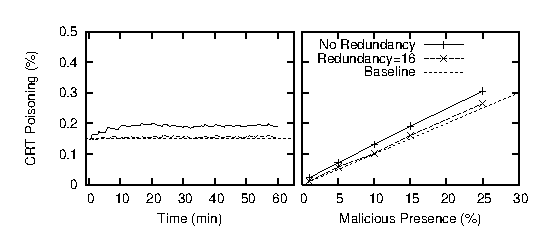
\includegraphics{graphs/crtPoisoning}}
\caption{\CRT poisoning without redundant routing and with
  16-path redundancy.  (a) Time graph of \CRT poisoning for 15\% malicious
  presence.  (b) Steady-state \CRT poisoning for different malicious
  presence levels.}
\label{fig:crtPoisoning}
\end{figure}

\begin{figure*}
\begin{center}
\centerline{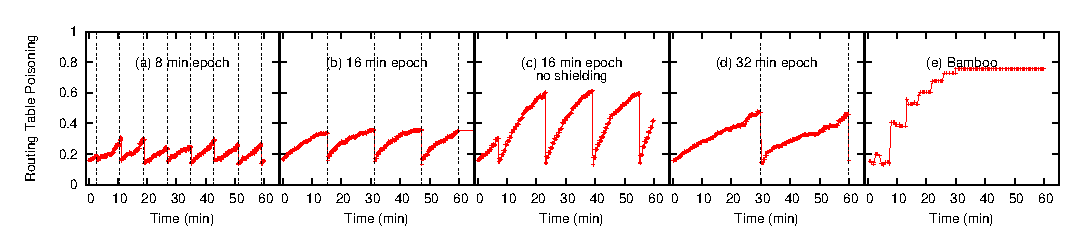
\includegraphics{graphs/timeGraph.eps}}
\caption{Routing-table poisoning vs.\ Time for 15\% malicious
fraction.}
\label{fig:timeGraph}
\end{center}
\end{figure*}

For both systems, we use a network topology based on the extended King
data set~\cite{Gummadi2002}, a commonly used realistic topology of a wide
variety of Internet
hosts.  We use the default values~\cite{Rhea2004} for Bamboo 
system parameters: the leaf-set size is 32 with a leaf-set update
interval of 10 sec; the \PRT is updated every 30 sec and keep-alive
pings are sent to all neighbors every 30 sec.  In terms of Maelstrom, nodes form $G=256$ churn
groups.  For all experiments, we set the randomness service timestep
duration to be $T/G$, where $T$ is the epoch length.

The threat model implemented in our attack simulations is structured
around a set of colluding malicious nodes conspiring to maximize the
routing-table poisoning in the entire population.
Malicious nodes hijack all routing state update messages that arrive at
them or pass through them, responding
with references to nodes from their malicious collective.
We give the adversary full
knowledge of every good node's routing state, to approximate an
adversary that has used traffic analysis to infer such state.  As a
result, the adversary can give responses to lookups
that will have the greatest impact on a given victim's routing table.  
Furthermore, when faced with multiple node candidates for an entry, good nodes always
choose the adversary's candidate, to approximate an adversary who can
successfully fool victims about its network measurements (Section~\ref{sec:eclipses}).
We discuss
our choice of threat model, as well as alternative weaker models in Section~\ref{sec:discussion}.


\SubSection{Routing state poisoning}

To evaluate Maelstrom's resistance to poisoning, we first study the
resistance to poisoning of the \CRT under induced churn, since the \CRT forms the baseline of the
``sawtooth'' behavior we hope to instill in the system
(Figure~\ref{fig:sawtooth}).  Then we evaluate the ability of the \PRT
to resist poisoning and to perform successful lookups.

We use the algorithmic simulator with $50,000$ nodes
under  attack. Figure~\ref{fig:crtPoisoning}(a) shows 
\CRT poisoning vs.\ time with 15\% malicious nodes in the population. 
Figure~\ref{fig:crtPoisoning}(b) shows the steady-state \CRT poisoning
for varying fractions of malicious presence in the population.  Both
graphs show experiments with and without 16-way redundant routing. We see that
poisoning remains closer to the fraction of malicious population with
redundancy; e.g., with 15\% malicious population, steady-state poisoning
hovers around 16\% with 16-way redundancy, and around 20\% without.
This is not surprising, since greater redundancy ensures a higher
probability of successful lookup routing, which means a greater
likelihood that a node updating its \CRT will receive a response from
the correct node it is probing.

We now turn to the \PRT itself, measuring its poisoning levels as a
function of malicious presence and epoch length. We use the same
experimental setup as above, with $50,000$ nodes out of which 15\% are
malicious. Figures~\ref{fig:timeGraph}(a), (b), and (d) show the
average \PRT
poisoning with time for nodes belonging to a single churn group in
Maelstrom, for epoch lengths of 8, 16, and 32 minutes.  We isolate a
single churn group to show how poisoning levels are affected by non-staggered
induced churn.
Dips in the graph indicate
the group's epoch boundaries, where nodes in the churn group reset their \PRT to their
\CRTNext (Section~\ref{sec:design}).  Longer epoch lengths allow the \PRT poisoning to increase.  This matches well
the intuition illustrated in Figure~\ref{fig:sawtooth}. 
In contrast, Bamboo (Figure~\ref{fig:timeGraph}(e)) poisoning 
continuously increases until a high saturation point around 80\%, more
than 5 times the baseline malicious presence of 15\%. 

To separate out the benefits obtained through row shielding alone, we
plot in Figure~\ref{fig:timeGraph}(c) one instance of the time graphs
(for 16-min epochs)
without row shielding.  The slope of the ``sawtooth'' pattern in this
figure matches Bamboo more closely, and is certainly steeper than the
equivalent scenario with
row shielding, in Figure~\ref{fig:timeGraph}(b).

\begin{figure}
\centerline{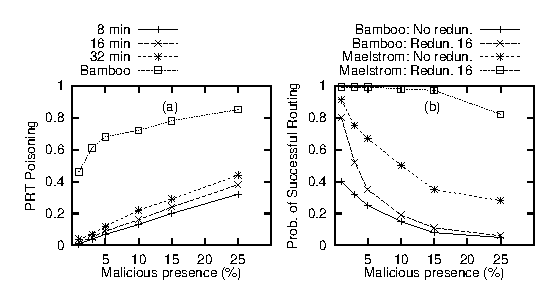
\includegraphics{graphs/prtPoisoning}}
\caption{\PRT security characteristics vs.\ malicious presence in the
  population. (a) Routing-table poisoning for different Maelstrom epoch lengths and for Bamboo.
  (b) Probability of successful lookup delivery for different redundancy
  levels for Bamboo and Maelstrom.}
\label{fig:prtPoisoning}
\end{figure}

Figure~\ref{fig:prtPoisoning}(a) supplies a broader view of the system's
behavior, over varying malicious presence in the population,
looking at the average \PRT poisoning over all good nodes (not just a
single churn group as above).
Bamboo yields great poisoning amplification to the adversary, especially
at low malicious fractions, while Maelstrom
maintains poisoning close to the baseline. Specifically, for up to 5\%
malicious nodes, Bamboo suffers from between 6 and
46 times greater poisoning than Maelstrom, depending on epoch length.
As above, the level of
poisoning in Maelstrom grows as the epoch length increases, since the
adversary can then increase her foothold in the good nodes'
routing tables for longer time periods.

Figure~\ref{fig:prtPoisoning}(b) shows the
actual probability that a lookup over the \PRT will reach its
destination -- as opposed to being intercepted and abused by the
adversary -- for an epoch length of 16 mins. 
Maelstrom does better than Bamboo in all cases. The difference is more pronounced for
low malicious presence; as malicious presence increases, even if
poisoning does not increase from its baseline, it can hinder lookups due
to their multi-hop nature.

To separate out the contributions of induced churn from redundant
routing, Figure~\ref{fig:prtPoisoning}(b) also plots successful lookups
when they are performed redundantly over the \PRT as well.  At 16-way
redundancy, Bamboo success drops rapidly as malicious presence tops 5\%, whereas
Maelstrom manages nicely, staying barely below 100\% success for low
malicious presence and achieving over 80\% success even when
malicious presence reaches 25\%.  This reinforces our earlier point:
without periodic resets of the optimized routing table, even
redundancy cannot
save lookups from adversarial tampering.

\begin{figure*}
\centerline{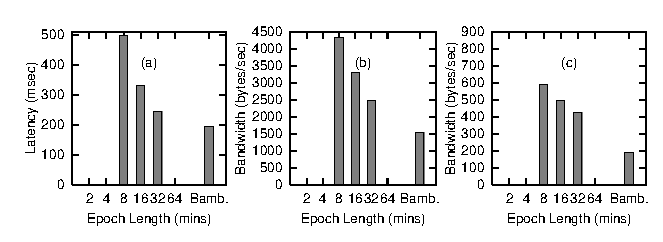
\includegraphics{graphs/simPerformance}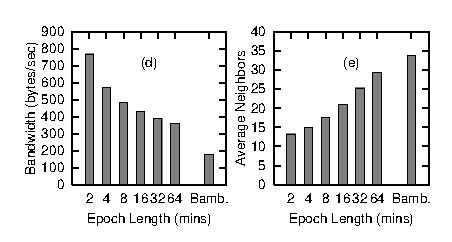
\includegraphics{bw_results/bwneighbors}}
\caption{Performance measurements as a function of epoch length,
  compared to Bamboo. (a) Lookup latency from algorithmic simulator
  ($50,000$ nodes); (b) \& (c) Maintenance bandwidth from the algorithmic
  simulator, $50,000$ and 500 nodes respectively; (d) Maintenance
  bandwidth from the implementation (500 nodes); and (e) Average number of neighbors
  per node from the implementation (500 nodes).}
\label{fig:performance}
\end{figure*}


\SubSection{Performance}

In this section we measure the performance overhead of induced churn on
Maelstrom. We conduct the experiments in the absence of attacks, since
Maelstrom is a proactive system that does not change mode of operation
in reaction to attack evidence.

Figure~\ref{fig:performance} collects performance measurements for
3-hour (simulated time) runs of Maelstrom and Bamboo in algorithmic simulation and on an
emulated network.  Figure~\ref{fig:performance}(a) shows the average network 
latency for successful lookups in a simulated population of $50,000$
nodes.  Latency increases as epoch length decreases, since routing state
optimizations have less time to complete before a table reset.  Bamboo
completes those optimizations and consequently exhibits the best (lowest) latency. 

Figures~\ref{fig:performance}(b), (c), and (d) compare per-node average maintenance
bandwidth under simulation with $50,000$ nodes, $500$ nodes, and on
an emulated network of $500$ nodes respectively.  Measurements include
bandwidth incurred by maintaining, pinging for liveness, and updating
three routing tables in Maelstrom, rather than the single routing table
in Bamboo.  Larger
populations fill up nodes' routing tables more, so the per-node
bandwidth overhead due to periodic node pings and routing-table updates
increases.  Furthermore, shorter epoch lengths incur more frequent
repopulations of \CRTNext from scratch, increasing bandwidth
consumption. The trends in simulation and on emulation are
similar. However, the algorithmic
simulator tends to overestimate maintenance costs slightly, since it does not
model optimizations such as suppressing liveness pings when other
traffic is observed, which are present in the actual implementation.
Nevertheless, even for short epochs and large populations, Maelstrom's bandwidth
requirements are well below the tolerance of even home users behind
dial-up modems.

Figure~\ref{fig:performance}(e) shows the average number of
neighbors for different epoch lengths on the full implementation at the
end of the 3-hour experiment. This graph also demonstrates how
induced churn can cut neighbor discovery short, as well as poisoning, which can potentially increase latencies
but moderates bandwidth increases.


We conclude by examining the
randomness server.  If
every node in a churn group contacts the server
individually, the server's access link must sustain a stream of
$(\mathit{Population}/\mathit{EpochLength})$ certificates.
$50,000$ nodes with a 2-minute epoch would incur a total of about 0.5 Mbps for
1-KByte 
randomness certificates, which
is trivial for even moderate services.  All requests concern the
same few certificates at any time, served from main memory, so the load
of about
$400$ requests per second is well below typical limits of off-the-shelf
web servers.  Furthermore, in practice nodes in a churn group can
disseminate a randomness certificate amongst themselves, reducing both
overheads on the server even more.  Finally, with 256 churn groups, the
server must compute two new certificates per second; even with
$2048$-bit signing keys, this is well within the capabilities of commodity processors.






\Section{Discussion}
\label{sec:discussion}

We now turn to the challenges
facing Maelstrom on its path from research prototype to real-world deployment.

\SubSection{The Randomness Service}
Our design includes a source of trusted, timed randomness to
ensure the unpredictability of node identifiers. This source of randomness could also help with load
balancing, topology formation, leader election, auctions, etc.
Maelstrom implements this functionality as a 
central, globally trusted service. Compared to other approaches to the
problem of secure routing that rely on certification authorities, a
central randomness server is simpler to implement, to prove correct, and
to audit; however, the randomness service makes the overlay more reliant
on service availability, since it
effectively ``clocks'' overlay progress.  Furthermore, centralized
components of either type can raise trust and reliability concerns.
In the context of the Maelstrom randomness service, we
can alleviate some of these concerns via \emph{accountability},
\emph{replication}, and \emph{redundancy}.

First, to make the service more accountable, we can provide its users with
assurances that issued random numbers are unpredictable to all parties
within given bounds. Users could periodically perturb the service pseudo-random
number generator by submitting to it new seeds that are incorporated in
subsequent number generation.  Similar techniques have been used in
verifiable secret sharing~\cite{Pedersen1991}, to ensure that no
participant in the protocol can bias collectively computed random
numbers.

Second, replication can improve availability, e.g., for times when a
randomness server is unreachable by certain clients.  Replicas of the
randomness server need only share a secret seed for their pseudo-random
functions, and be loosely time-synchronized.  Both requirements are
easy to meet, especially compared to the burden of replicating
the more complex central live identity certification
authorities, whose state changes and must be propagated to replicas as
identities are issued or revoked.

Third, redundancy can narrow
the need for global trust.  With
redundancy, there are multiple, independent randomness servers, each distributing its
own separate randomness source.  Overlay nodes compute their IDs by
hashing together random numbers from all or many servers.  Verifiers can
validate IDs computed from those sources of randomness that they trust,
ignoring others; as long as at least one randomness server it trusts has
been used in an ID computation, a validator can accept that overlay
ID. Such approaches have been used before for highly available time
stamping services~\cite{Ansper2001}.

In future work, we hope to combine all three techniques with
timeline entanglement~\cite{Maniatis2002b} to distribute the
functionality of the randomness service completely, when
absolutely no shared servers can be tolerated. 


\SubSection{Adversary Bestiary}
\label{sec:diversityEnforcement}
Our adversary model is comprised of a conspiracy of malicious nodes that
collude to poison the routing tables of all the good nodes
in the overlay.  Although an ``attack everyone'' threat model is an
important one, there are other
more directed threat models that may also be interesting, which we only
briefly mention due to space limitations.  Instead of everyone, the adversary could
attack a particular key (to cripple a resource) or a particular node (to
cripple a service operator), as a
destination (to intercept incoming requests) or as a source of traffic
(to produce spam or to hijack normal responses).  Though more
limited in scope, such attacks could
allow a weaker adversary to concentrate her resources on a specific target.

One aspect of the adversary that we have not included in our analysis and
design is her capacity for increasing her presence in the system, for
example via \emph{Sybil}
identities, which are forged or otherwise spoofed identities.
By imposing a 3-way handshake on every IP-level session, we  ensure
that a node's IP address is a legitimate one, or one that the node can
spoof easily (e.g., within a /24 network). The use of a 3-way handshake, however, only restricts a node to assuming an IP address that it can spoof easily. In Maelstrom, we
have explored the enforcement of \emph{IP address diversity}, by which nodes
limit the number of representatives from each such easy-to-spoof address
set in their routing tables.  Diversity enforcement successfully thwarts spoofing
adversaries from amplifying their poisoning potential.  However it also
penalizes overlay participants from large organizations (e.g., student
computers at a large university);  while an overlay can accommodate
nodes from such non-diverse address spaces, it cannot reach its fully
optimized connectivity, which would be possible with a uniform address
distribution.

\SubSection{Utility}
Maelstrom offers a trade-off between the performance costs and the
security benefits of the overlay (refer to Figure~\ref{fig:performance}).
The performance cost depends
on lookup latency due to sub-optimal routing, and maintenance
bandwidth due to periodic, unpredictable churn.  There can also be
associated application costs if, for example, the overlay is used as a
distributed hash table to store data; then induced churn incurs a
bandwidth cost due to data migration. The epoch length allows
the system to be tuned according to the relative utility assigned to
performance and security by the
application using the overlay.  On one hand, 
for distributed file systems and databases the 
cost of migrating data
across nodes could be high, and induced churn
may be inappropriate. On the other hand, for
monitoring, query processing, or content distribution, the
cost is considerably lower since smaller, fewer, or expendable data items are
involved, and high periodic churn can be sustained to
provide greater resistance to poisoning.

Along a different axis, for some applications the quality of the average-case state of
good nodes' routing tables is less important than avoiding the worst case.
For instance, in a preservation application such as
PAST~\cite{Rowstron2001b}, content is not refreshed by its publisher
into the repository. Instead, it is inserted once and then migrated
among replicas as the system churns.  In such an application, arriving \emph{ever}
at a system state in which all replicas of a given document
are controlled by the adversary is detrimental, since it gives the
adversary the opportunity to tamper with the document permanently.  Reducing
churn then is an absolute goal, since it reduces the likelihood of ever
achieving such a worst-case state.  Induced churn is inappropriate for
such applications.  Contrast this to the common case of monitoring,
repositories, and communication overlay applications, which require
clients to  refresh stored content periodically.  In
such applications, it is more important to reduce the average-case
routing-table poisoning, since this measure determines whether clients can reach the
desired content or not, and has no bearing on the content's eventual
survival.  Induced churn is appropriate in such settings and, in
adversarial environments, it is indispensable.

\SubSection{Migrating data}
To continue to be useful, Maelstrom must ensure that the data inserted
remain available to clients. An obvious solution to the problem is
to replicate data amongst some set of nodes (usually a subset of the
leaf set called the replica set) as discussed by 
Rhea et al~\cite{Slowness-OpenDHT}. In this case, every $put$ under a key $k$
would contact the nodes in the replica set and return success only if
the put succeeds on a quorum of the replica set. Any $get$ would then
contact the replica set and read values from a quorum. By choosing these
quora appropriately, we can ensure that applications can retrieve the
most up-to-date data. However, the presence of induced churn implies
that nodes fail periodically. It is quite possible that all the nodes in
the replica set may churn before handing data over to any of the
``nearby'' nodes. To handle this case, we can have each node maintain
pointers to its ``ancestors'' -- the set of nodes that previously owned
the keys that the node currently owns. Any lookup on keys that have a
valid ``ancestor'' is rerouted to the ancestor. Nodes periodically
synchronize with their ancestors and remove the association between
ancestors and a key for each synchronized key.

\SubSection{Reliance on IP addresses}
A question may arise about the reliance of Maelstrom for its benefits
on current IP addressing.
For instance, how easily would
our design carry over to IPv6, given its larger address space?

Maelstrom relies for its protection against eclipse attacks on there
being a hierarchical structure in IP addresses, whereby higher-order
bits are fixed per organization, and assigned centrally (currently by
the IANA), whereas lower-order bits are assigned to end hosts by the
organization itself.  Such higher-order bits are used to choose churn
groups in a manner that cannot be biased by the adversary.  In that
sense, we have termed higher-order bits
``unspoofable'' (Section~\ref{sec:staggering}): a malicious end host
cannot change those address bits in traffic it originates and still
participate in arbitrary two-way IP
exchanges without collusion from the Internet's governing agencies.
To the extent that this requirement holds with IPv6 addresses, Maelstrom
is compatible with the newer IP protocol.  Note, however, that the
definition of how many high-order address bits make up the
``unspoofable'' part of an address would have to adapt to current addressing
policies.

Similarly, Maelstrom may rely on IP address structure to combat Sybil
attackers, that is, adversaries who create many IP addresses with the
low-order address bits within their organizations, hoping to sway the
balance of adversarial presence in the overlay.  As described in Section~\ref{sec:diversityEnforcement},
diversity enforcement may help.  Again, the number of high-order bits
that define equivalence classes among nodes for the purposes of
diversity enforcement must match the deployment policies of the current
IP protocol.  For IPv4, enforcing diversity within a routing table among
the 24 high-order bits appears sufficient.



\Section{Related Work}

Security analysis of structured overlays and 
other peer-to-peer systems have recently appeared in the
literature~\cite{Douceur2002,Sit2002,Wallach2002}, recognizing 
routing-table poisoning as a serious threat.
Castro et al.~\cite{Castro2002} proposed the first comprehensive
solution to the problem in the context of
Pastry~\cite{Rowstron2001}. Their proposal relied on a central certification authority
issuing rate-limited ID certificates, on dual
routing tables (one for optimized and one for secure routing),
and on routing failure detectors.  Singh et al.~\cite{Singh2004} extended this work to handle
\emph{eclipse} attacks in general overlays (structured and unstructured)
by enforcing low in- and out-degree of vertices in the overlay graph via
anonymous auditing.  Low in- and out-degrees mean that malicious nodes cannot
insert themselves to arbitrarily many good nodes' routing tables.
These two approaches make heavy use of an ID certification authority.
Though perfectly
reasonable for instance in enterprise environments enjoying wide
trust, such powerful and complex globally
trusted components are harder to justify in more open settings.
Maelstrom is inspired by this trailblazing work, but seeks to relax the reliance
on a powerful and complex central entity. Compared to an ID certification
authority that verifies ``real-world'' credentials, issues
rate-limited ID certificates, and monitors and distributes revocations, our
timed randomness service is a simpler component that can be more easily
proved correct, debugged, audited, and distributed.

Recent work by Awerbuch and
Scheideler~\cite{Awerbuch2004,Scheideler2005} shares
many of the intuitions behind Maelstrom and even proves some of them
under certain assumptions. The authors' designs use verifiable secret sharing to allow
groups of nodes to generate random identifiers for newcomers, and to enforce
limited identifier lifetimes.  The approach though very complex and as
yet unimplemented to our knowledge, is proved 
robust when adversarial nodes and good nodes are limited in their join
and departure rates from the overlay.  In contrast, Maelstrom 
enforces this rate limitation in the protocol itself and
off-loads the task of random number generation to a shared service.
Furthermore, it concentrates on extending implemented structured overlays, giving
priority to retaining the optimizations that make these overlays practical.
We have yet to formally prove the robustness of our techniques, but our
simpler design has allowed us to implement them and evaluate them
experimentally for some adversaries.

Our basic techniques have been used before in different contexts:
rate-limited routing-table updates to ease load spikes under
churn~\cite{Rhea2004}, increased unpredictability to thwart adversarial
behavior that relies on predictability~\cite{Kc2003}, and periodic
resets to rejuvenate a degrading system~\cite{Candea2004,Castro2000}.



\Section{Conclusion}

In this work, we have motivated, designed, and experimentally evaluated
\emph{induced churn}, a defense against routing-table poisoning in structured
overlays.  Induced churn combines periodic routing-table reset,
unpredictable identifiers, and rate-limited updates to protect such
overlays from adversaries who wish to inflate their presence in good nodes'
routing tables beyond what their presence in the population as a
whole would justify.  We have demonstrated induced churn by implementing Maelstrom, an
extension to a real distributed hash table in wide use
today~\cite{Rhea2004}.
We show that induced churn can thwart adversaries who could otherwise intercept almost all
lookups, even with a very limited presence.
Yet, it retains many of the benefits of optimized structured
overlays, making tunable the trade-off between resistance to poisoning and efficient routing.

In future work, we hope to understand better the strengths and
limitations of induced churn in realistic adversarial environments
through experimentation in real deployments, and through further analysis.
Today, Bamboo forms the basis for a number of research and production projects
deployed in the wild, including OpenDHT~\cite{Rhea2005}, a shared
infrastructure for DHT-based applications.  We hope to assist the
maintainers of OpenDHT with the deployment of the Maelstrom extensions,
so as to investigate how induced churn behaves, even when data migration
is necessary.

Finally, we believe that the need for common sources of unpredictability
is becoming increasingly important in loosely coupled distributed
systems.  We hope to study further designs proposed in the
literature, or those proposed here, for a massively replicated or
fully-distributed timed randomness
service, hoping to provide a \emph{randomness dial tone} that can help
safeguard distributed systems in the ever more
dangerous internetworks they occupy.

\Section{Acknowledgments}

We would like to thank Sean Rhea for his invaluable help in extending
Bamboo with the Maelstrom extensions, David Wagner for his
thoughtful comments on earlier versions of this paper, our shepherd Dan
Wallach, and the anonymous
reviewers for their feedback.  Tyson Condie and Joe Hellerstein are
partially supported by NSF grants (contract numbers 0209108 and
0225660), and by a gift from Microsoft Corporation.



\bibliographystyle{latex8}
%\bibliographystyle{plain}
\bibliography{bibliography}

\end{document}


% LocalWords:  DHT filesharing DHTs overlay's IP DHT's fallback timestep
% LocalWords:  timesteps
